% Aqui começa o capítulo de Metodologia (ou Desenvolvimento, conforme o template)
% Vamos usar "Metodologia" como título, pois parece mais alinhado com o conteúdo
% que você descreveu para o Capítulo 3, mas mantendo o label do template.
\chapter{Metodologia}\label{chp:desenvolvimento} % Alterei o título para "Metodologia"

Este capítulo detalha a metodologia empregada para o desenvolvimento e validação do \textit{framework} computacional proposto para a segmentação semântica de tecido canceroso em WSIs de biópsias de câncer de próstata. A abordagem metodológica é organizada em etapas sequenciais, desde a aquisição e preparação dos dados até o treinamento, monitoramento, análise de resultados e inferência dos modelos de DL.

\section{Visão Geral do \textit{Framework}}\label{sec:met_visao_geral}

A metodologia desenvolvida nesta dissertação estrutura-se em seis etapas principais: (1) Aquisição e Preparação dos Dados, (2) Pré-processamento Adicional e Geração de Conjuntos, (3) Treinamento dos Modelos de DL, (4) Monitoramento do Treinamento, (5) Análise de Resultados, e (6) Inferência e Aplicação. Este fluxo de trabalho visa garantir a sistematicidade, a eficiência e a replicabilidade do processo de segmentação semântica de câncer de próstata em WSIs.

A \Figura{fig:framework_diagrama} apresenta um diagrama esquemático que ilustra a interconexão e a sequência dessas etapas principais. O processo inicia-se com a inspeção e organização das WSIs e suas anotações, seguido pela extração de \textit{patches} e aplicação de filtros para seleção de ROI. O pré-processamento inclui normalização de cor e aumento de dados (\textit{augmentation}). A etapa de treinamento envolve a exploração de diferentes arquiteturas (CNNs, \textit{Transformers}) e o treinamento final de um \textit{ensemble} híbrido, utilizando ferramentas para monitoramento de métricas. Finalmente, os modelos treinados são avaliados e integrados em uma aplicação para inferência em novas imagens. Cada uma dessas etapas é detalhada nas seções subsequentes deste capítulo.

% Figura do Pipeline (Diagrama do Framework)
\begin{figure}[!htb] % Posicionamento sugerido: aqui, topo ou fundo.
    \centering
    % Comando para incluir a imagem do pipeline
    \includegraphics[width=\textwidth]{figuras/pipeline.png} % Usar \textwidth para tentar ocupar a largura da página, ajuste se necessário.
    \caption[Diagrama do \textit{framework} Metodológico]{Visão geral do \textit{framework} computacional \textit{end-to-end} proposto. O diagrama ilustra as seis etapas principais: Aquisição de \textit{patches} (incluindo análise de artefatos, criação de banco de dados, \textit{image patching} e criação de máscara binária), pré-processamento (com a limpeza da base de câncer, normalização de cor, \textit{augmentation} da menor classe, geração de conjuntos de treinamento, validação e teste, \textit{sanity check} dos resultados e \textit{Zip} e \textit{Upload} dos dados para ambiente de computação de alto processamento), Investigação de \textit{Learning Rate} para a base de imagens, treinamento do \textit{ensemble}, monitoramento, otimização da participação de cada modelo treinado no \textit{ensemble} e inferência (com análise de resultados e aplicação). O diagrama ilustra também os pontos no processo onde existe a geração de metadados, que são informações necessárias para replicabilidade dos resultados.}
    \label{fig:framework_diagrama} % Label para referenciar a figura
\end{figure}

\section{Aquisição e Preparação dos Dados}\label{sec:met_aquisicao_dados}

A qualidade e a preparação adequada dos dados são fundamentais para o sucesso de qualquer projeto de aprendizado de máquina, especialmente em domínios complexos como a patologia digital. Nesta pesquisa, foram utilizados quatro conjuntos de dados distintos para treinar, validar e testar a capacidade de generalização do \textit{framework} proposto: uma base proprietária proveniente de uma colaboração internacional e três bases públicas renomadas na literatura (DIAGSET, CATCH e CAMELYON16).

\subsection{Conjunto de Dados e Inspeção Inicial}\label{subsec:met_dataset_inspecao}

A seguir, são detalhadas as características, origens e protocolos de anotação de cada base de dados utilizada.

\subsubsection{Base de Dados Proprietária (Chile)}\label{subsubsec:dataset_chile}

O conjunto de dados principal deste estudo compreende 104 \textit{Whole Slide Images} (WSIs) de biópsias de câncer de próstata, provenientes de 54 pacientes, fruto de uma colaboração com a Universidad de La Frontera (Chile). Todas as WSIs foram fornecidas no formato \texttt{\Sigla{\textit{Scanned Virtual Slide}}{SVS}} -- Slide virtual escaneado, em tradução livre. Este é um formato comumente associado a scanners de lâminas e visualizável através de softwares específicos como o Aperio ImageScope \cite{AperioImageScope}, que foi utilizado para a inspeção inicial das imagens e anotações. É importante notar que o número de WSIs excede o número de pacientes pois, para alguns casos, diferentes patologistas realizaram anotações sobre a mesma lâmina digital, ou múltiplas regiões de uma mesma lâmina foram anotadas como entradas separadas, gerando assim múltiplos arquivos de anotação e, consequentemente, sendo tratadas como WSIs distintas no contexto da nossa pipeline de processamento. As respectivas anotações médicas, realizadas por patologistas experientes, foram disponibilizadas em formato XML. Todas as imagens e anotações foram devidamente anonimizadas, sendo os pacientes identificáveis apenas por um ID único.

A \Figura{fig:wsi_exemplo_aperio} apresenta um exemplo de uma WSI visualizada no software Aperio ImageScope, onde é possível observar a lâmina histológica em baixa magnificação (miniatura à direita), uma região de interesse em maior detalhe, e as sobreposições das anotações realizadas pelos patologistas. A inspeção inicial revelou a grande dimensão desses arquivos de imagem (Gigabytes), e a complexidade das anotações, reforçando a necessidade de um pipeline de processamento robusto.

% Figura do Aperio ImageScope (sua Figura 3 original)
\begin{figure}[!htb] 
    \centering
    % Substitua 'figuras/aperio_imagescope_exemplo.png' pelo nome/caminho correto da sua imagem
    \includegraphics[width=\textwidth]{figuras/aperio.PNG} 
    \caption[Exemplo de WSI e Anotações no Aperio ImageScope]{Exemplo de uma WSI de biópsia de próstata visualizada no software Aperio ImageScope. Observam-se as anotações de ROIs realizadas por patologistas, com contornos em vermelho indicando áreas de câncer e contornos em verde indicando áreas não cancerosas.}
    \label{fig:wsi_exemplo_aperio} 
\end{figure}

A inspeção inicial das imagens e, particularmente, dos arquivos XML de anotação, revelou desafios inerentes ao processo de marcação manual realizado por múltiplos patologistas. Como o processo de anotação de WSIs é laborioso e consome tempo considerável, a tarefa é frequentemente distribuída entre diversos profissionais para reduzir a carga de trabalho individual. Essa prática, embora necessária, pode introduzir variabilidade, especialmente na escolha exata das cores ou na delineação precisa das Regiões de Interesse (ROIs).

Visando mitigar essa variabilidade em nosso conjunto de dados, foi instituída pela junta médica responsável pelas anotações uma padronização de cores para as diferentes classes de tecido. A \Figura{fig:padrao_cores_anotacoes_medicas} ilustra o padrão de cores definido, onde, para a tarefa de segmentação binária de tecido prostático de interesse nesta dissertação (câncer vs. não câncer), o \textbf{Vermelho} foi designado para anotações de "Positivo" (câncer) e o \textbf{Verde} para "Negativo" (não câncer). Outras cores foram designadas para artefatos ou outros tipos de ROI não diretamente utilizados neste trabalho.

% Figura do Padrão de Cores
\begin{figure}[!htb] 
    \centering
    % Substitua 'figuras/padrao_cores_anotacoes.png' pelo nome/caminho correto da sua imagem
    \includegraphics[width=0.7\textwidth]{figuras/medical_standards.png} 
    \caption[Padrão de cores para anotações médicas.]{Convenção de cores estabelecida pela junta médica para a anotação das ROIs nas WSIs. Para este estudo, as cores de interesse primário são o vermelho (Positivo/Câncer) e o verde (Negativo/Não Câncer).}
    \label{fig:padrao_cores_anotacoes_medicas} 
\end{figure}

Apesar da tentativa de padronização, a inspeção detalhada dos arquivos XML revelou que, para a classe "Não Câncer", alguns patologistas ocasionalmente utilizavam tonalidades de verde ligeiramente diferentes. Isso resultava em códigos de cor distintos dentro do atributo \texttt{LineColor} do arquivo XML para a mesma classe semântica, como pode ser observado no exemplo da \Figura{fig:exemplo_xml_linecolor}, onde o valor "65280" (um tom de verde) é usado para "Não Câncer", enquanto em outras anotações poderia aparecer um valor como "65408" para a mesma finalidade. Essa pequena variação, se não tratada, dificultaria a criação de um algoritmo genérico para extrair as coordenadas das ROIs baseado em um único código de cor para "Não Câncer".

% Figura do Exemplo de XML de Anotação
\begin{figure}[!htb] 
    \centering
    % Substitua 'figuras/exemplo_xml_anotacao.png' pelo nome/caminho correto da sua imagem
    \includegraphics[width=0.9\textwidth]{figuras/xml_example.png} 
    \caption[Exemplo de estrutura XML de anotação com variação de LineColor.]{Trecho de um arquivo XML de anotação ilustrando como as regiões são definidas. Destaca-se o atributo \texttt{LineColor}, onde "255" (tipicamente vermelho) pode representar "Câncer", enquanto valores como "65280" (um tom de verde) representam "Não Câncer". A variabilidade nesses códigos de cor para a mesma classe semântica (Não Câncer) necessitou de tratamento específico.}
    \label{fig:exemplo_xml_linecolor} 
\end{figure}

Para resolver essa incerteza nos códigos de cor, foi criada uma tabela de mapeamento (descrita na \Secao{subsec:met_banco_dados}) que relaciona cada arquivo SVS com os códigos de cor específicos utilizados para "Câncer" e "Não Câncer" naquela lâmina. Isso permitiu que os algoritmos de processamento de imagens utilizassem os códigos de cor corretos como parâmetros de entrada para cada WSI individualmente.

Outro desafio significativo encontrado durante a inspeção manual foi a presença de \textbf{anotações ambíguas}. Em algumas WSIs, para determinados pacientes, a mesma região tecidual foi identificada e anotada tanto como "Câncer" (vermelho) quanto como "Não Câncer" (verde) por diferentes anotações ou patologistas, como ilustrado na \Figura{fig:anotacoes_ambiguas_exemplo}. Tal comportamento introduz uma incerteza fundamental na classificação daquele pixel ou região, o que poderia degradar significativamente o processo de aprendizado da rede neural se esses dados fossem utilizados diretamente. Para contornar este problema e garantir a qualidade do conjunto de treinamento, foram implementadas regras nos algoritmos de processamento de \textit{patches} para identificar e ignorar sistematicamente as regiões com anotações dúbias ou sobrepostas contraditoriamente.

% Figura das Anotações Ambíguas
\begin{figure}[!htb] 
    \centering
    % Substitua 'figuras/anotacoes_ambiguas.png' pelo nome/caminho correto da sua imagem
    \includegraphics[width=0.7\textwidth]{figuras/ambiguous_image.PNG} 
    \caption[Exemplo de anotações ambíguas em uma WSI.]{Ilustração de uma região em uma WSI onde ocorreram anotações ambíguas, com a mesma área tecidual sendo delimitada tanto como "Câncer" (contornos vermelhos) quanto como "Não Câncer" (contornos verdes). Regiões com tal sobreposição contraditória foram ignoradas durante a geração dos \textit{patches} de treinamento.}
    \label{fig:anotacoes_ambiguas_exemplo} 
\end{figure}

\subsubsection{DIAGSET (Câncer de Próstata)}\label{subsubsec:dataset_diagset}

O \textit{DiagSet} é um conjunto de dados público recente voltado para a classificação histopatológica de câncer de próstata \cite{Koziarski2024DiagSet}. A base foi construída a partir de material escaneado durante diagnósticos laboratoriais padrão e posteriormente anonimizado. As amostras biológicas consistem em biópsias por agulha (\textit{needle biopsies}) fixadas em formalina, emblocadas em parafina e coradas com Hematoxilina e Eosina (H\&E).

A digitalização das lâminas foi realizada utilizando um scanner digital \textit{Hamamatsu C12000-22} com uma lente objetiva de 40x, resultando em uma resolução de 0.25 $\mu m$/pixel. O formato nativo dos arquivos é o NDP (\textit{NanoZoomer Digital Pathology}).

O conjunto de dados é subdividido em três partes principais, sendo o subconjunto \textbf{DiagSet-A} o de maior relevância para tarefas de segmentação supervisionada abordadas neste trabalho. O DiagSet-A contém WSIs totalmente anotadas por um grupo de histopatologistas experientes. As anotações definem regiões poligonais classificadas em 9 classes possíveis, incluindo: fundo do escaneamento, fundo do tecido (estroma sem relevância), tecido saudável normal, artefatos de aquisição e os graus de Gleason de 1 a 5. Para fins de treinamento neste estudo, as classes de Gleason foram mapeadas para a classe positiva ("Câncer"), enquanto tecido saudável e fundo foram mapeados para a classe negativa ("Não Câncer"). O volume de dados anotados no DiagSet-A totaliza 428 WSIs, fornecendo uma base robusta para validação cruzada com dados de uma população demograficamente distinta (Polônia) da base proprietária.

\subsubsection{CAMELYON16 (Câncer de Mama)}\label{subsubsec:dataset_camelyon}

O dataset \textit{CAMELYON16} origina-se de uma competição de grande impacto na área de patologia digital (\textit{Cancer Metastases in Lymph Nodes Challenge 2016}), focada na detecção de metástases de câncer de mama em linfonodos sentinela \cite{bandi2019detection}. Embora o foco histológico primário deste estudo seja próstata, a inclusão do CAMELYON16 permite validar a robustez da arquitetura do \textit{framework} em uma tarefa de detecção de metástase padrão-ouro na literatura.

A base é composta por 399 WSIs obtidas de dois centros médicos nos Países Baixos: o \textit{Radboud University Medical Center} (RUMC) e o \textit{University Medical Center Utrecht} (UMCU). Esta característica multicêntrica introduz variações importantes de digitalização, uma vez que o RUMC utilizou o scanner \textit{Pannoramic 250 Flash II} (3DHISTECH) e o UMCU utilizou o \textit{NanoZoomer-XR} (Hamamatsu Photonics), enriquecendo a variabilidade de cor e resolução (0.243 $\mu m$/pixel e 0.226 $\mu m$/pixel, respectivamente) nos dados de teste.

O \textit{ground truth} desta base é considerado de altíssima qualidade. As anotações das metástases (macrometástases e micrometástases) foram realizadas manualmente por estudantes sob supervisão de patologistas e, crucialmente, validadas através de coloração imuno-histoquímica (IHC) para citoqueratina em cortes seriados. O uso da IHC permitiu resolver incertezas diagnósticas e garantir que o conjunto de treinamento e teste não contivesse falsos negativos, tornando-o ideal para benchmarks de sensibilidade e especificidade.

\subsubsection{CATCH (Câncer de Pele Canino)}\label{subsubsec:dataset_catch}

O dataset \textit{CATCH}, apresentado por Wilm et al. \cite{Wilm2022CATCH}, oferece uma perspectiva única de patologia comparativa ao disponibilizar WSIs de tumores cutâneos caninos. A inclusão desta base no presente estudo tem como objetivo estratégico avaliar a robustez e a flexibilidade do \textit{framework} proposto ao aplicá-lo em um domínio biológico completamente distinto. Testar a metodologia em imagens de tecido animal, que possuem características histológicas próprias e diferem do tecido humano prostático, permite validar a capacidade de generalização do método, demonstrando que a arquitetura desenvolvida é agnóstica ao tipo de tecido e não está restrita apenas à anatomia humana.

O conjunto é composto por 350 WSIs coradas com H\&E, abrangendo sete subtipos de tumores cutâneos (como melanoma, carcinoma de células escamosas e mastocitoma). As imagens foram digitalizadas utilizando scanners lineares \textit{Leica ScanScope CS2} e \textit{Leica AT2}, predominantemente com resolução de 0.2533 $\mu m$/pixel (40x).

O diferencial desta base reside na granularidade das anotações: foram fornecidos 12.424 polígonos de anotação abrangendo 13 classes histológicas distintas. Além dos subtipos tumorais, há anotações detalhadas para estruturas de tecido não neoplásico, como epiderme, derme, subcutâneo, osso, cartilagem, além de classes específicas para necrose e inflamação. Essas anotações foram realizadas utilizando a plataforma \textit{SlideRunner} e validadas por patologistas veterinários, garantindo alta consistência nos rótulos (\textit{labels}).


\subsection{Análise e Detecção Automática de Artefatos}\label{subsec:met_analise_artefatos}

A presença de artefatos em lâminas histológicas digitais — tais como dobras de tecido, bolhas de ar, regiões fora de foco, marcas de caneta e poeira — representa um desafio significativo para o treinamento de modelos de DL. Estes elementos não contêm informação biológica relevante e podem introduzir ruído nos dados, levando a falsos positivos ou à degradação da capacidade de generalização do modelo \cite{Weng2024GrandQC}.

Para mitigar este problema de forma sistemática e automatizada, adotou-se neste trabalho o \textit{framework} \textbf{GrandQC}, uma solução abrangente para controle de qualidade em patologia digital proposta recentemente por \textcite{Weng2024GrandQC}. A escolha desta ferramenta justifica-se pela sua robustez na segmentação multiclasse de artefatos e pela sua validação extensiva em diversos centros de patologia e sistemas de digitalização.

\subsubsection{Arquitetura e Metodologia do GrandQC}

O método GrandQC opera através de uma abordagem de segmentação semântica baseada em Redes Neurais Convolucionais (CNNs). O \textit{pipeline} implementado consiste em dois módulos sequenciais baseados na arquitetura \textbf{U-Net++} \cite{Zhou2018}, utilizando codificadores \textit{EfficientNet-B0}\cite{Tan2019EfficientNet} pré-treinados no banco de dados \textit{ImageNet} \cite{Deng2009} para extração de características.

\begin{enumerate}
    \item \textbf{Módulo de Detecção de Tecido:} O primeiro estágio processa a WSI em baixa resolução para gerar uma máscara binária inicial, distinguindo o tecido biológico do fundo da lâmina (vidro). Esta etapa otimiza o processamento subsequente, restringindo a busca de artefatos apenas às regiões contendo tecido.
    
    \item \textbf{Módulo de Detecção de Artefatos:} O segundo estágio opera nas regiões de interesse definidas pelo módulo anterior. Este modelo realiza uma segmentação multiclasse para identificar e delimitar categorias específicas de artefatos, incluindo: desfoque (\textit{out-of-focus}), dobras de tecido (\textit{folds}), bolhas de ar, bordas da lâmina, marcas de caneta e corpos estranhos/manchas escuras.
\end{enumerate}

\subsubsection{Implementação Computacional e Geração de Máscaras}

Para a operacionalização desta etapa no \textit{framework} proposto, desenvolveu-se um \textit{script} de automação em Python integrado à biblioteca \texttt{OpenSlide} \cite{OpenSlide} para manipulação eficiente de imagens piramidais. O processamento foi configurado para utilizar a versão do modelo GrandQC treinada com uma resolução de 1.5 $\mu m$/pixel (aproximadamente equivalente a uma magnificação de 7x), o que oferece um equilíbrio entre precisão na detecção de pequenos artefatos e eficiência computacional, de acordo como descrito no artigo original \cite{Weng2024GrandQC}.

O fluxo de processamento implementado segue as seguintes etapas para cada WSI do conjunto de dados:

\begin{enumerate}
    \item \textbf{Inferência de Tecido:} A WSI é carregada e processada pelo modelo de detecção de tecido (MPP=10) para gerar uma máscara global de ROI.
    \item \textbf{Inferência de Artefatos:} As regiões de tecido são divididas em \textit{patches} de $512 \times 512$ pixels. O modelo de detecção de artefatos realiza a inferência em cada \textit{patch}, classificando os pixels nas classes de artefatos ou tecido limpo.
    \item \textbf{Pós-processamento e Exportação:} As máscaras de predição dos \textit{patches} são reconstruídas (\textit{stitching}) para formar uma máscara de artefatos completa da lâmina.
\end{enumerate}

Como resultado final desta etapa, além das máscaras de segmentação visuais (arquivos PNG), o algoritmo foi programado para extrair os contornos dos artefatos detectados e exportá-los em formato \textbf{GeoJSON}. Estes arquivos vetoriais contêm as coordenadas exatas dos polígonos de artefatos em relação à dimensão original da imagem. 

Esta estratégia permitiu a integração direta com a etapa de geração de \textit{patches} de treinamento: durante a extração das regiões de interesse, o algoritmo consulta o arquivo GeoJSON correspondente e descarta automaticamente quaisquer \textit{patches} que apresentem sobreposição significativa com áreas de artefatos, garantindo a pureza e qualidade dos dados fornecidos à rede neural.


\subsection{Banco de Dados para Gerenciamento de Imagens}\label{subsec:met_banco_dados}

Para viabilizar o gerenciamento robusto e reprodutível do fluxo de processamento massivo das WSIs, implementou-se uma arquitetura de orquestração baseada em um banco de dados relacional \textit{SQLite} \cite{sqlite}. A escolha do \textit{SQLite} fundamentou-se em três pilares estratégicos para a pesquisa: (1) \textbf{Portabilidade}, visto que o banco de dados consiste em um único arquivo em disco, facilitando o compartilhamento do estado exato dos experimentos; (2) \textbf{Facilidade de Implementação}, dispensando a configuração de servidores dedicados; e (3) \textbf{Persistência de Metadados}, garantindo que cada \textit{patch} gerado possa ser rastreado até sua imagem de origem e aos parâmetros exatos utilizados em sua criação.

O gerenciamento é realizado por meio de um script que interage com uma tabela de controle criada dinamicamente com base em \textit{tags} experimentais (e.g., \texttt{DATABASE\_V1}). A estrutura desta tabela foi projetada para atuar simultaneamente como um registro histórico e uma fila do tipo \Sigla{\textit{First-In, First-Out}}{FIFO} \cite{cormen2022introduction}.

A metodologia de gerenciamento opera em duas fases distintas e sequenciais, assegurando a integridade dos dados:

\begin{enumerate}
    \item \textbf{Fase de Ingestão e Verificação (\textit{Ingest}):} 
    Nesta etapa, o algoritmo varre os diretórios de imagens (\texttt{IMAGES\_\{TAG\}}) e anotações (\texttt{ANNOTATIONS\_\{TAG\}}). Novos casos identificados são inseridos no banco de dados com o status inicial \texttt{'TO BE PROCESSED'}. Durante a ingestão, o sistema realiza verificações de sanidade (\textit{sanity checks}), como a validação da existência de arquivos pareados (imagem e XML) e, opcionalmente, a presença de arquivos GeoJSON para filtragem avançada de artefatos. É nesta fase que códigos de cor específicos para cada WSI (como é o caso da base de dados Chile) são associados ao registro da imagem, contornando a variabilidade de anotação entre patologistas.
    
    \item \textbf{Fase de Processamento e Orquestração:} 
    O \textit{script} atua como um despachante. Ele consulta o banco de dados em busca de registros com status pendente. Para cada caso, o sistema:
    \begin{itemize}
        \item Recupera os parâmetros de configuração definidos via variáveis de ambiente (\textit{.env}), tais como tamanho da janela (\texttt{WINDOW\_SIZE}), passo de corte (\texttt{STRIDE}) e limiares de tecido. Isso garante que a configuração experimental esteja dissociada do código, facilitando a replicação.
        \item Executa o algoritmo de \textit{patching} como um sub-processo independente. Essa estratégia de isolamento impede que uma falha de memória ou erro de execução em uma imagem específica corrompa o fluxo principal ou interrompa o processamento da fila e também aumenta a velocidade do processo como um todo.
        \item Atualiza o registro no banco de dados com métricas de execução (tempo de processamento, quantidade de \textit{patches} de câncer e não-câncer gerados) e altera o status para \texttt{'COMPLETED'} ou \texttt{'FAILED'}, registrando logs de erro na coluna \texttt{COMMENTS} quando necessário.
    \end{itemize}
\end{enumerate}

Esta abordagem orientada a banco de dados oferece vantagens críticas para a reprodutibilidade científica do \textit{framework}:

\begin{itemize}
    \item \textbf{Resiliência e Retomada:} O sistema permite a interrupção e reinício do processamento a qualquer momento sem perda de trabalho. Em caso de falhas externas (e.g., queda de energia, desconexão do \textit{Google Colab}), o algoritmo retoma a execução a partir da próxima imagem com status \texttt{'TO BE PROCESSED'}, eliminando redundâncias.
    \item \textbf{Rastreabilidade Granular:} Cada experimento possui sua própria tabela e conjunto de parâmetros imutáveis registrados por imagem. Isso permite auditorias futuras para verificar exatamente quais configurações (e.g., \texttt{MATCH\_PERCENTAGE}, \texttt{STRIDE}) foram usadas para gerar um determinado conjunto de treinamento.
    \item \textbf{Adaptação Dinâmica:} O sistema permite o tratamento individualizado de lâminas. Parâmetros críticos, como as cores das anotações (\texttt{CANCER\_COLOR}), são lidos dinamicamente do banco para cada WSI durante a execução, permitindo que o \textit{framework} processe, em uma única execução, um \textit{dataset} heterogêneo composto por anotações de diferentes fontes.
\end{itemize}

A estrutura detalhada dos campos da tabela de controle e seus tipos de dados encontra-se documentada no Apêndice \ref{ap:esquema_banco_dados} (ver \Tabela{tab:ap_esquema_database}).

\section{Corte de Imagens (\textit{Patching}) e Geração de Máscaras}\label{sec:met_corte_imagens}

Devido às dimensões exorbitantes das WSIs (frequentemente na ordem de gigapixels), o processamento direto por redes neurais profundas é computacionalmente inviável. Para contornar essa limitação, adotou-se a estratégia de particionamento da imagem em recortes menores, denominados \textit{patches}. Este processo foi implementado através de um \textit{pipeline} dividido em três sub-processos lógicos: (1) Orquestração via Banco de Dados (descrito na \Secao{subsec:met_banco_dados}), (2) Abstração e Gerenciamento de Anotações, e (3) Engenharia de Corte e Filtragem.

A execução deste fluxo é controlada por um script que integra os módulos de manipulação de dados e o motor de processamento paralelo.

\subsection{Gerenciamento de Imagens e Anotações (Data Handlers)}

A falta de padronização nos formatos de arquivos em patologia digital impõe um desafio de interoperabilidade. Para solucionar isso, o módulo de ingestão de dados foi construído seguindo o padrão de projeto \textit{Template Method}. Foi definida uma classe base abstrata (\texttt{BaseHandler}) que estabelece o contrato para o carregamento de dados, delegando a implementação da lógica de \textit{parsing} para subclasses especializadas via polimorfismo.

O sistema seleciona dinamicamente o manipulador adequado (\texttt{Handler Dispatch}) com base na extensão dos arquivos de entrada, suportando:
\begin{itemize}
    \item \textbf{SVS/XML:} Para lâminas Aperio com anotações em XML.
    \item \textbf{NDPI/NDPA:} Para lâminas Hamamatsu.
    \item \textbf{TIFF/JSON:} Para formatos genéricos ou datasets como CAMELYON16 e CATCH.
\end{itemize}

Uma funcionalidade crítica implementada nesta etapa é a limpeza geométrica das anotações. Antes do corte, o algoritmo identifica e remove regiões de ambiguidade espacial, onde polígonos de "Câncer" e "Não Câncer" possam se sobrepor inadvertidamente, utilizando operações de diferença de conjuntos da biblioteca \textit{Shapely}. Isso garante que o \textit{ground truth} fornecido à rede neural seja geometricamente consistente.

\subsection{Engenharia de Corte e Otimização}

A etapa de corte (\textit{patching}) opera sob duas premissas: maximizar a extração de informação relevante e minimizar o custo computacional. Para isso, o motor de processamento (\texttt{patch\_engine.py}) emprega as seguintes estratégias:

\begin{enumerate}
    \item \textbf{Varredura Otimizada por \textit{Bounding Box}:} Em vez de percorrer a totalidade da lâmina (que é majoritariamente composta por fundo branco), o algoritmo calcula a caixa delimitadora (\textit{bounding box}) global de todas as anotações presentes. A geração da grade de coordenadas restringe-se a esta área de interesse, reduzindo drasticamente o tempo de busca.
    
    \item \textbf{Paralelismo em CPU:} A extração dos \textit{patches} é distribuída entre múltiplos processos (\texttt{multiprocessing.Pool}), utilizando todos os núcleos de CPU disponíveis para leitura concorrente da WSI via biblioteca \textit{OpenSlide}.
    
    \item \textbf{Definição de Grade:} Os parâmetros de corte são definidos pelas variáveis de ambiente \texttt{WINDOW\_SIZE} e \texttt{STRIDE}. Quando o valor definido pelo \texttt{STRIDE} é inferior ao \texttt{WINDOW\_SIZE}, existe uma sobreposição entre \textit{patches} adjacentes. Esta sobreposição acaba por propiciar um aumento da densidade de dados disponíveis para treinamento, conforme sugerido por \textcite{Fan2020}.
\end{enumerate}

\subsection{Critérios de Filtragem e Seleção de ROI}

Para garantir que apenas dados de alta qualidade componham o \textit{dataset}, cada \textit{patch} candidato é submetido a uma cadeia rigorosa de três filtros de aprovação:

\begin{enumerate}
    \item \textbf{Filtro de Conteúdo Tecidual:} Visa eliminar imagens que contêm majoritariamente fundo de lâmina (vidro). O algoritmo converte o \textit{patch} para o espaço de cor HSV e aplica uma limiarização de Otsu no canal de Saturação. A máscara resultante passa por operações morfológicas de abertura (kernel elíptico $3\times3$ para remoção de ruído) e fechamento (kernel elíptico $7\times7$ para preenchimento de lacunas). O \textit{patch} é rejeitado se a proporção de tecido for inferior a \texttt{TISSUE\_PERCENTAGE}. Vale destacar aqui que os valores para os Kernels das operações morfológicas foram obtidos de forma empírica e não são, portanto, valores ótimos, sendo ambos passíveis de otimização. Todavia, os valores de 3 e 7 se adequaram bem ao hardware utilizado durante os experimentos.
    
    \item \textbf{Filtro de Relevância de Anotação:} Verifica a intersecção espacial entre a área do \textit{patch} e os polígonos de anotação médica. Um \textit{patch} é classificado e salvo apenas se a sobreposição com a anotação da classe alvo exceder o limiar \texttt{MATCH\_PERCENTAGE}, podendo ser alterado de 0 a 1.
    
    \item \textbf{Filtro de Artefatos (Opcional):} Caso um arquivo GeoJSON de artefatos esteja disponível (gerado pela etapa de detecção descrita na \Secao{subsec:met_analise_artefatos}), o sistema calcula a intersecção do \textit{patch} com as regiões de artefato (e.g., dobras, caneta). Se a cobertura do artefato exceder um limiar definido na política de artefatos (\texttt{artifact\_policy.yaml}), o \textit{patch} é descartado para evitar a contaminação do modelo com ruído.
\end{enumerate}

\subsection{Geração de Máscaras Binárias e Persistência}\label{subsec:met_mascaras_binarias}

Para cada \textit{patch} aprovado nos critérios de filtragem, o \textit{framework} gera uma máscara de segmentação binária correspondente, que serve como \textit{ground truth} para o treinamento supervisionado.

A máscara é construída rasterizando-se os polígonos de anotação médica projetados nas coordenadas locais do \textit{patch}. Conforme ilustrado na \Figura{fig:patch_e_mascara_binaria}, pixels correspondentes à classe "Câncer" são codificados com valor 1 (visualizados em branco), enquanto pixels de fundo, estroma não anotado ou classe "Não Câncer" são codificados com valor 0 (preto).

% Figura do Patch e sua Máscara Binária
\begin{figure}[!htb] 
    \centering
    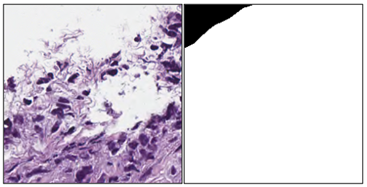
\includegraphics[width=0.6\textwidth]{figuras/image_plus_mask.png} 
    \caption[Exemplo de \textit{patch} de WSI e sua máscara binária correspondente.]{Ilustração do resultado do processo de engenharia de corte. \textbf{(Esquerda)} Um \textit{patch} de tecido prostático (H\&E) aprovado pelos filtros de tecido e anotação. \textbf{(Direita)} A máscara binária gerada, onde a região tumoral anotada é representada em branco (valor 1) e o restante em preto (valor 0).}
    \label{fig:patch_e_mascara_binaria} 
\end{figure}

Os pares de imagem e máscara são salvos em formato PNG (\Sigla{\textit{Portable Network Graphics}}{PNG}) para evitar perdas por compressão. A nomenclatura dos arquivos segue o padrão \texttt{<CLASSE>\_PATIENT\_<ID>\_<X>\_<Y>\_<HASH>\_<TIMESTAMP>}, assegurando rastreabilidade total da origem espacial e temporal de cada amostra.

\section{Pré-processamento Adicional e Geração de Conjuntos}\label{sec:met_preproc_conjuntos}

\subsection{Normalização de Cor}\label{subsec:met_norm_cor} % Este é o label que você já usava
Conforme discutido na \Secao{subsubsec:fund_norm_cor}, a variabilidade de coloração H\&E representa um desafio significativo em patologia digital. Para mitigar esse efeito no presente trabalho, foi aplicada a técnica de normalização de cor proposta por Reinhard a todos os \textit{patches} gerados. Essa escolha foi também motivada pelos avanços recentes na área, como apresentado por Shen et al.~\cite{Shen2022}, cujo trabalho reforça a importância de estratégias robustas de normalização para o aprendizado de características invariantes à coloração em lâminas histológicas.

A implementação prática desta etapa envolveu primeiramente a definição de estatísticas de cor de referência ($\mu_{ref}, \sigma_{ref}$) no espaço CIE LAB. Para evitar o viés que poderia ser introduzido pela escolha de uma única imagem de referência, estas estatísticas globais foram calculadas como a média das médias e a média dos desvios padrão de um conjunto representativo de \textit{patches}. Especificamente, um \textit{patch} foi selecionado aleatoriamente de cada um dos 54 pacientes do conjunto de dados para compor este conjunto de referência, garantindo a representatividade da variabilidade interpaciente. Os valores de $\mu_{ref}$ e $\sigma_{ref}$ calculados (aproximadamente [161.1, 146.3, 114.2] para as médias L\*, a\*, b\* e [39.6, 5.8, 5.9] para os desvios padrão, respectivamente, conforme detalhado na \Tabela{tab:parametros_inferencia_framework}) foram então salvos em um arquivo no formato \Sigla{\textit{JavaScript Object Notation}}{JSON}. 

Este arquivo JSON com as estatísticas de referência tornou-se uma dependência crucial do \textit{framework}, assegurando que a mesma transformação de normalização de cor pudesse ser aplicada de forma consistente a todos os \textit{patches} processados, tanto durante a fase de treinamento dos modelos quanto, fundamentalmente, durante a etapa de inferência em novas WSIs. Esta consistência é vital para a reprodutibilidade dos resultados e para o desempenho generalizável dos modelos de DL.

\subsection{Geração de Amostras de Treino, Validação e Teste}\label{subsec:met_geracao_amostras}
Os conjuntos de dados de treino, validação e teste foram criados utilizando o script \texttt{4\_crossfold.py}. Foi empregada uma estratégia de validação cruzada estratificada por grupos (\textit{StratifiedGroupKFold} do pacote scikit-learn \cite{Pedregosa2011}), com 5 \textit{folds}. Esta abordagem garante que todos os \textit{patches} de um mesmo paciente pertençam exclusivamente a um único conjunto (treino, validação ou teste) dentro de um \textit{fold}, prevenindo o vazamento de dados e fornecendo uma estimativa mais realista do desempenho do modelo em dados não vistos. Para os experimentos exploratórios iniciais, visando agilidade, foi utilizada uma subamostra dos pacientes (aproximadamente 50\% do total), e a divisão para cada \textit{fold} seguiu uma proporção aproximada de 80\% para treino, 10\% para validação e 10\% para teste. Para garantir a replicabilidade na geração dos subgrupos, foi utilizada uma semente (\textit{seed}) de 42.

\subsection{Image Augmentation}\label{sec:metodologia_augmentation} 
O desbalanceamento de classes entre regiões de câncer e não câncer é comum em datasets de patologia. Para contornar este problema e aumentar a diversidade dos dados, foi aplicada \textit{image augmentation} na classe minoritária (após identificação) de cada \textit{fold} de treinamento, até que houvesse um equilíbrio numérico de amostras com a classe majoritária. O \textit{framework} implementado permite cinco tipos de \textit{augmentations}: transformações puramente geométricas (rotação horizontal, vertical, aleatória), adição de ruído gaussiano e variação aleatória de contraste, brilho e saturação (\textit{color jittering}). É importante notar que a aplicação do \textit{color jittering} ocorre após a etapa de normalização de cor de Reinhard (descrita na \Secao{subsec:met_norm_cor}). Embora a normalização de Reinhard vise padronizar a aparência cromática global, a subsequente aplicação controlada de \textit{color jittering} tem como objetivo aumentar a robustez do modelo a pequenas variações de cor residuais ou inerentes ao processo de aquisição, incentivando o aprendizado de características morfológicas mais resilientes a tais flutuações, em vez de uma "despadronização" descontrolada do que foi previamente normalizado.

Diferentemente da prática comum de aplicar \textit{augmentation} dinamicamente durante o treinamento, neste \textit{framework} optou-se por realizar esta etapa no pré-processamento. Esta decisão visa dois objetivos principais: (1) \textbf{Controle e Análise Detalhada:} Permite um controle explícito sobre os tipos e a quantidade de \textit{augmentations} aplicadas. As imagens aumentadas são salvas com uma nomenclatura específica (\texttt{<tipo>\_<ID\_paciente>\_<metadados>\_aug\_<tipo\_augmentation>}), facilitando investigações futuras sobre o impacto de cada técnica de \textit{augmentation} nas métricas do modelo e garantindo a reprodutibilidade exata das transformações. (2) \textbf{Eficiência de Processamento no Treinamento:} Ao realizar a \textit{augmentation} uma única vez, o tempo de processamento durante os múltiplos ciclos de treinamento dos modelos é reduzido, especialmente relevante ao experimentar com diversas arquiteturas e hiperparâmetros. Embora bibliotecas de treinamento ofereçam controle sobre \textit{augmentation on-the-fly}, a abordagem de pré-geração foi considerada mais alinhada com os objetivos de análise detalhada e reprodutibilidade deste \textit{framework}.

\subsection{Sanity Check e Preparação para Treinamento em Ambiente Virtual}\label{subsec:met_sanity_zip}
Antes de iniciar o treinamento, uma etapa de \textit{sanity check} foi implementada para inspecionar a qualidade dos conjuntos de dados gerados, verificando a quantidade de pixels por classe e a ausência de contaminação de pacientes entre os conjuntos de treino, validação e teste de cada \textit{fold}.
Considerando a inviabilidade de treinar os modelos em máquinas locais devido aos recursos computacionais exigidos, os diretórios de \textit{patches} de treino, validação e teste foram comprimidos em arquivos ZIP individuais para cada \textit{fold} e enviados para o ambiente \textit{Google Colab Pro}. Esta compressão agiliza significativamente o processo de transferência de dados em comparação com o upload de milhares de arquivos de imagem individualmente.

\section{Treinamento dos Modelos de DL}\label{sec:met_treinamento_dl}

\subsection{Investigação do LR}\label{subsec:met_lr_finder}
O LR, que é a taxa de aprendizagem do modelo, é um dos hiperparâmetros mais críticos no treinamento de redes neurais, influenciando diretamente a velocidade de convergência e a qualidade do mínimo encontrado pela função de perda. Para estimar uma taxa de aprendizado inicial segura e eficaz para os modelos deste trabalho, foi empregada a técnica de \textit{learning rate range test}, popularizada como \textit{learning rate finder} \cite{Smith2017}. Este método consiste em treinar o modelo por um pequeno número de iterações, começando com um LR muito baixo e aumentando-o exponencialmente a cada lote, enquanto se registra a perda.

A \Figura{fig:lr_finder_exemplo} ilustra um exemplo típico da saída deste procedimento, onde a perda é plotada em função da taxa de aprendizado em escala logarítmica. Observa-se que, para taxas de aprendizado muito baixas, a perda diminui lentamente ou permanece estagnada. À medida que o LR aumenta, a perda começa a diminuir mais rapidamente, atingindo um ponto de declive máximo (indicado na figura), que é frequentemente sugerido como uma boa taxa de aprendizado inicial. Após este ponto, com o aumento contínuo do LR, a perda pode começar a oscilar e, eventualmente, divergir, indicando que a taxa de aprendizado se tornou excessivamente alta.

% Figura do Learning Rate Finder
\begin{figure}[!htb] 
    \centering
    % Substitua 'figuras/lr_finder_plot.png' pelo nome/caminho correto da sua nova imagem
    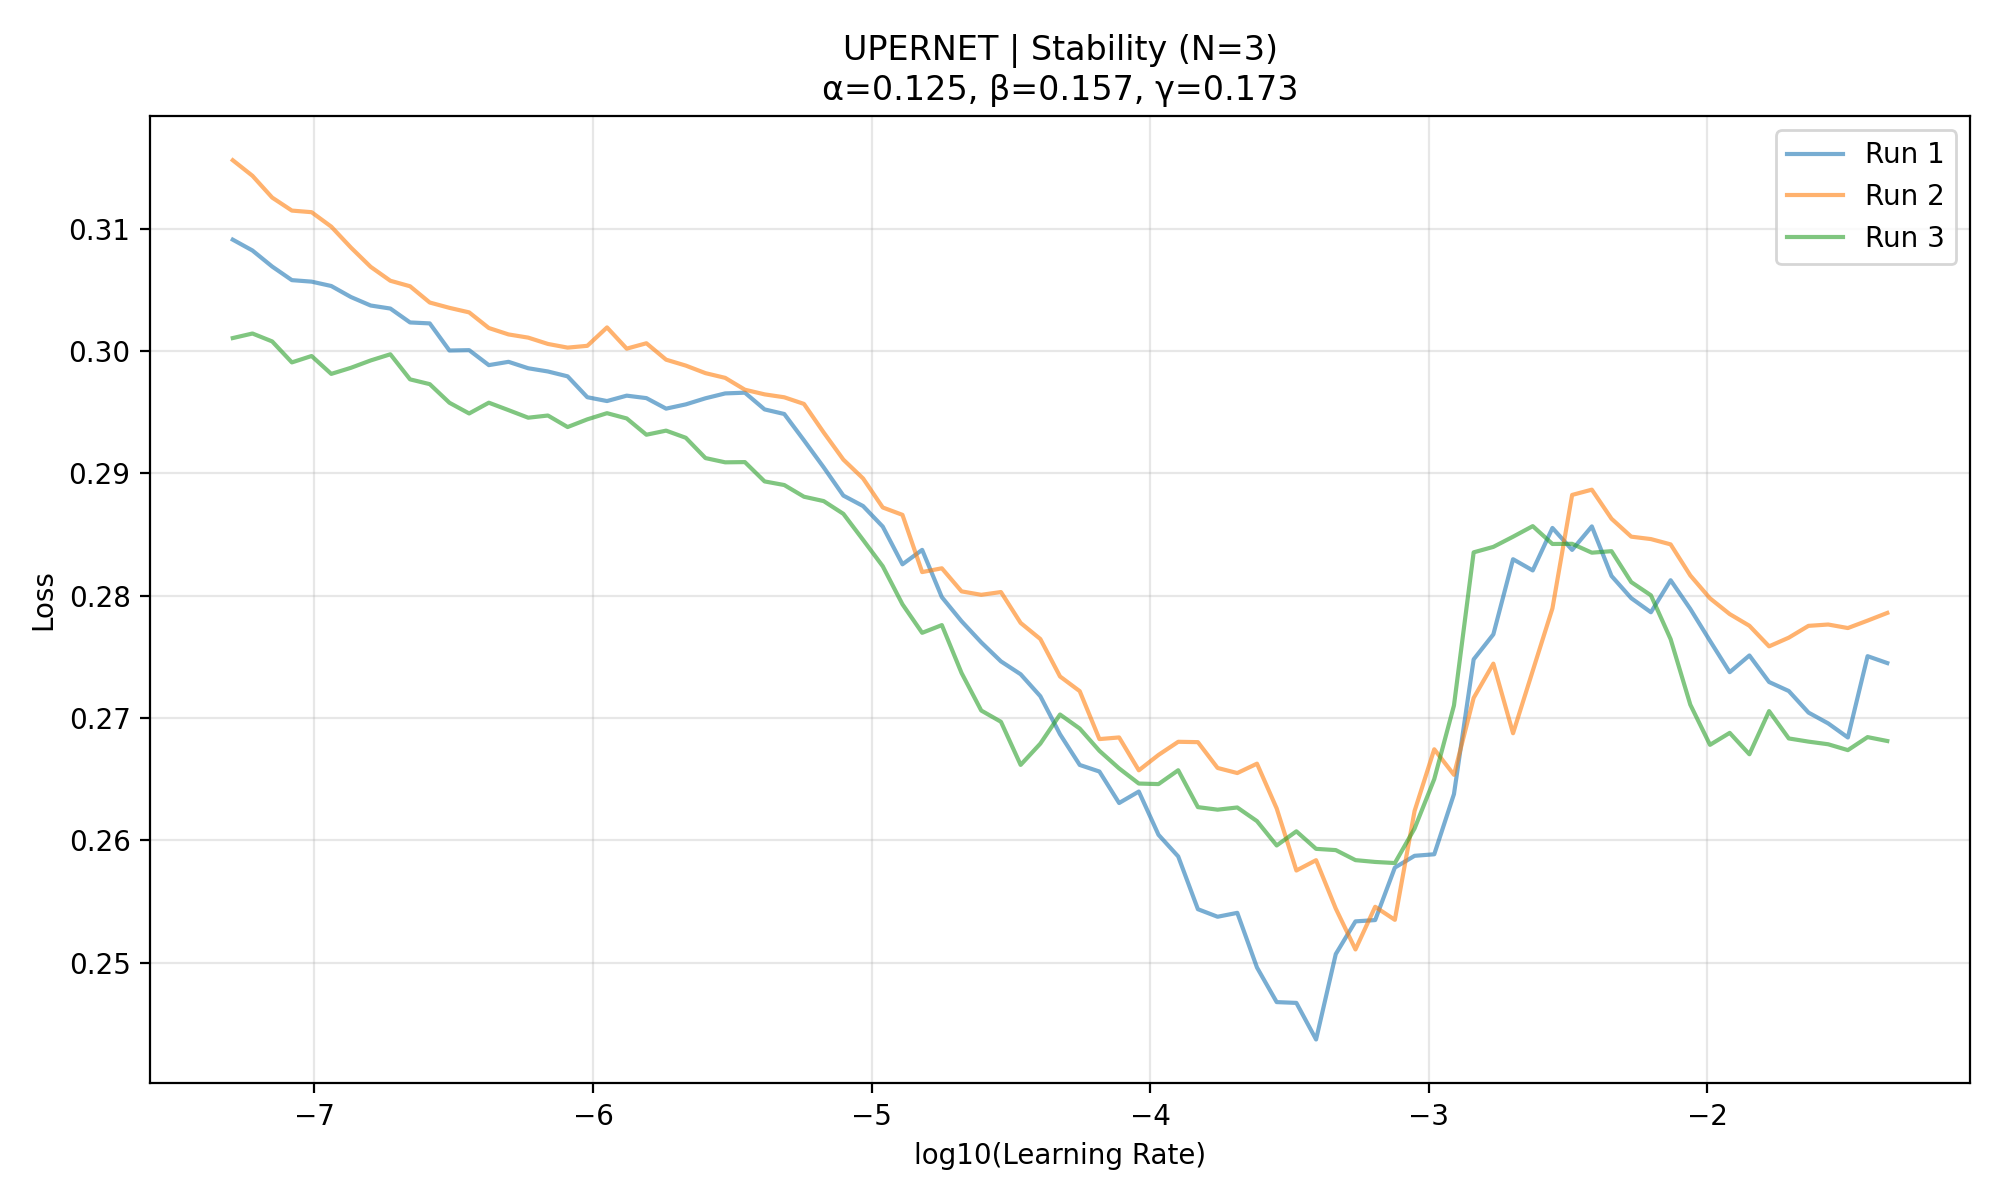
\includegraphics[width=0.7\textwidth]{figuras/LR_finder.png} 
    \caption[Exemplo da Saída do Teste de Faixa da Taxa de Aprendizado (\textit{Learning Rate Finder})]{Gráfico ilustrativo do resultado de um teste de faixa da taxa de aprendizado. A perda (\textit{Loss}) é plotada em função da taxa de aprendizado (\textit{Learning rate}) em escala logarítmica. O ponto vermelho indica a região de maior declive do gradiente, frequentemente sugerida como uma taxa de aprendizado inicial ótima (neste exemplo, 9.33E-04, embora para os modelos desta dissertação, valores próximos a 1E-5 tenham sido identificados como mais estáveis após pré-inicialização com ImageNet).}
    \label{fig:lr_finder_exemplo} 
\end{figure}

Simulações deste tipo, realizadas com as diversas arquiteturas de modelos utilizadas neste estudo (todas pré-inicializadas com pesos da ImageNet \cite{Deng2009}), indicaram consistentemente que, embora o ponto de declive máximo pudesse variar, uma taxa de aprendizado base mais conservadora, próxima de 1E-5, demonstrava ser um ponto de partida mais estável e eficaz para o início do treinamento, evitando divergências prematuras e permitindo uma convergência mais suave. Este valor foi, portanto, adotado como a taxa de aprendizado inicial para a maioria dos experimentos exploratórios.

\subsection{Arquiteturas e Configuração do Treinamento Exploratório}\label{subsec:met_arq_treino_exp}
Para a fase exploratória de identificação dos modelos e parâmetros mais promissores, foram adotadas diversas arquiteturas, abrangendo modelos baseados em \textit{Transformers} e modelos convolucionais.

Entre as arquiteturas baseadas em \textit{Transformers}, foram explorados: \textbf{SWIN Transformers} (com encoders \textit{tiny}, \textit{base} e \textit{large}) \cite{Liu2021}, \textbf{SegFormer} (com encoders MiT-B2, MiT-B3, MiT-B5) \cite{Xie2021}, e o \textbf{\Sigla{\textit{Dense Prediction Transformer}}{DPT}} (com encoder ViT-Base) \cite{Ranftl2021}.

Dentre os modelos predominantemente convolucionais, foram incluídos: \textbf{DeepLabv3+} (com encoders ResNet50, ResNet101 e ResNet152) \cite{Chen2018}, \textbf{UNET} (com encoder InceptionResNetv2) \cite{Ronneberger2015, Szegedy2017}, \textbf{UNET++} (com encoders ResNet50, ResNet101 e ResNet152) \cite{Zhou2018}, \textbf{\Sigla{\textit{Feature Pyramid Network}}{FPN}} (com encoders ResNet50, ResNet101 e ResNet152) \cite{Lin2017}, e a \textbf{\Sigla{\textit{Multi-Scale Attention Network}}{MANET}} (com encoder ResNet152) \cite{Fan2020}.

Com exceção dos encoders do SWIN Transformer, obtidos do ambiente HuggingFace \cite{HuggingFace}, as demais arquiteturas convolucionais e baseadas em \textit{Transformers}, bem como a vasta gama de \textit{encoders} pré-treinados, foram disponibilizados e utilizados através da biblioteca \Sigla{\textit{Segmentation Models PyTorch}}{SMP} \cite{Iakubovskii2019}. A escolha desta biblioteca foi estratégica, alinhando-se ao princípio de não reinventar implementações de arquiteturas já consolidadas e validadas pela comunidade científica, o que permite focar os esforços de pesquisa em outros aspectos do \textit{framework}.

A biblioteca SMP destaca-se por diversas características que facilitaram o desenvolvimento deste trabalho, incluindo uma \Sigla{\textit{Application Programming Interface}}{API} de alto nível que simplifica significativamente a criação e experimentação com diversas arquiteturas de segmentação e acesso a mais de 800 \textit{encoders} pré-treinados.
A utilização de uma biblioteca robusta e mantida ativamente pela comunidade, como a SMP, não apenas acelera o desenvolvimento, mas também garante maior confiabilidade e facilita a reprodutibilidade dos experimentos.

Nesta fase exploratória inicial, o desempenho das diversas arquiteturas e configurações de hiperparâmetros foi avaliado através de um processo de validação cruzada com 5 \textit{folds}. Conforme detalhado na \Secao{subsec:met_geracao_amostras}, estes \textit{folds} foram derivados de uma subamostra representativa dos pacientes, uma estratégia adotada para otimizar o tempo e os recursos computacionais durante esta etapa de prospecção intensiva de modelos. É crucial ressaltar que todos os pesos dos modelos (\textit{checkpoints}) obtidos nesta fase exploratória foram utilizados unicamente para fins de análise comparativa e seleção das arquiteturas mais promissoras. Consequentemente, esses \textit{checkpoints} foram descartados e não foram empregados diretamente na construção ou treinamento do \textit{ensemble} final, garantindo assim a independência entre a fase de exploração e a fase de construção e validação do modelo definitivo. Esta abordagem visa assegurar que a avaliação do \textit{ensemble} final seja realizada sobre modelos treinados especificamente para essa finalidade, utilizando o conjunto de dados completo, conforme será detalhado na \Secao{sec:res_treino_ensemble}.
O treinamento foi conduzido em ambiente \textit{Google Colab Pro}, utilizando GPUs com 15 GB de RAM, discos de 235.7 GB e memória RAM de 12.7 GB (expansível). Foi utilizada uma política de parada antecipada (\textit{early stopping}) com paciência de 5 épocas: se a métrica de perda (\textit{loss}) no conjunto de validação não apresentasse melhora por 5 épocas consecutivas, o treinamento era encerrado. Esta estratégia visou otimizar o uso dos créditos e limites de tempo do ambiente e evitar o \textit{overfitting} durante o treinamento.

A função de perda utilizada como guia foi uma combinação ponderada de duas métricas principais: \Sigla{\textit{Binary Cross-Entropy}}{BCE} e \textit{Dice Loss} (DL).

A BCE avalia o erro de classificação pixel a pixel, medindo a dissimilaridade entre a distribuição de probabilidade predita e a distribuição verdadeira. Para $N$ pixels em uma imagem ou lote, sendo $p_i$ a probabilidade predita pelo modelo para o pixel $i$ pertencer à classe positiva ("câncer") e $g_i$ o rótulo verdadeiro do \textit{ground truth} (1 para câncer, 0 para não câncer), a BCE é calculada como na \Equacao{eq:bce_formula}:
\begin{equation}\label{eq:bce_formula}
    \text{BCE} = \sum_{i=1}^{N} [g_i \log(p_i) + (1 - g_i) \log(1 - p_i)] \protect\footnote{Esta formulação da Entropia Cruzada Binária (BCE) representa o negativo da log-verossimilhança e, como tal, é maximizada. Na prática de otimização em \textit{deep learning}, onde se busca minimizar uma função de perda (\textit{loss function}), utiliza-se frequentemente o negativo desta expressão, ou seja, $-\sum_{i=1}^{N} [g_i \log(p_i) + (1 - g_i) \log(1 - p_i)]$. Muitos \textit{frameworks} implementam diretamente esta versão negativa como a \textit{loss} a ser minimizada.}
\end{equation}

A Dice Loss (DL) é derivada do Coeficiente de Dice e visa maximizar diretamente a sobreposição espacial entre a predição e a máscara real, sendo particularmente eficaz em tarefas de segmentação com desbalanceamento de classes \cite{Milletari2016}. Utilizando a formulação \textit{soft Dice} comum em treinamento, onde $p_i$ e $g_i$ são definidos como acima, a Dice Loss para uma classe específica é dada pela \Equacao{eq:dl_formula}:
\begin{equation}\label{eq:dl_formula}
    \text{DL} = 1 - \frac{2 \sum_{i=1}^{N} p_i g_i}{\sum_{i=1}^{N} p_i^2 + \sum_{i=1}^{N} g_i^2}
\end{equation}


A função de perda final utilizada neste trabalho combinou estas duas métricas, aplicando a Dice Loss separadamente para a classe "câncer" ($\text{DL}_{\text{câncer}}$) e para a classe "não câncer" ($\text{DL}_{\text{não-câncer}}$). Esta abordagem combinada, similar à utilizada por \textcite{Khened2021}, busca balancear a otimização da classificação pixel a pixel (via BCE) com a otimização da sobreposição espacial (via DL). A perda total é calculada como:
\begin{equation}\label{eq:loss_total_nova} % Novo label para esta versão da equação
    \text{loss} = \alpha \cdot \text{BCE} + \beta \cdot \text{DL}_{\text{câncer}} + \gamma \cdot \text{DL}_{\text{não-câncer}}
\end{equation}
onde BCE é calculado sobre a classe "câncer" (\Equacao{eq:bce_formula}), $\text{DL}_{\text{câncer}}$ e $\text{DL}_{\text{não-câncer}}$ são calculados usando a \Equacao{eq:dl_formula} para as respectivas classes (ajustando $p_i$ e $g_i$ para cada caso), e $\alpha, \beta, \gamma$ são pesos que balanceiam a contribuição de cada termo. Os pesos $\alpha, \beta, \gamma$ foram fixados em 0.5, 0.25 e 0.25, respectivamente, para todos os treinamentos exploratórios.

Após o treinamento de cada modelo em um determinado \textit{fold}, a avaliação no conjunto de teste correspondente requer a conversão das saídas brutas da rede (logits) em um mapa de probabilidades. Para esta tarefa, que no presente estudo envolve duas classes de saída ("câncer" e "não câncer"), a função \textbf{Softmax} \cite{Bishop2006} foi aplicada à camada final do modelo. Para um dado vetor de logits de saída $\mathbf{z} = (z_1, z_2, ..., z_C)$ para $C$ classes (onde $C=2$ neste caso), a probabilidade $p_c$ para cada classe $c$ é calculada como:

\begin{equation}\label{eq:softmax}
    p_c = \text{softmax}(\mathbf{z})_c = \frac{e^{z_c}}{\sum_{k=1}^{C} e^{z_k}}
\end{equation}

onde \( e \) é a base do logaritmo natural, \( e \approx 2{,}71828 \).

A função Softmax normaliza as saídas para que representem uma distribuição de probabilidade, ou seja, $p_c \in [0,1]$ e $\sum_{c=1}^{C} p_c = 1$. Embora uma função sigmóide \cite{Bishop2006} pudesse ser utilizada para a predição da classe "câncer" em um cenário binário, a escolha da Softmax com duas saídas foi mantida por facilitar a potencial extensão do \textit{framework} para problemas de segmentação multiclasse em trabalhos futuros, sem necessidade de alterar a arquitetura de predição do modelo. As probabilidades resultantes para a classe de interesse (câncer) são então utilizadas para a determinação do limiar de decisão.

Em vez de utilizar um limiar fixo padrão (\eg, 0.5) sobre essas probabilidades para binarizar a predição, optou-se por determinar um \textbf{limiar de decisão ótimo ($th^*$) dinamicamente}. Este procedimento visa maximizar uma métrica de segmentação de interesse, como o Coeficiente de Dice, no conjunto de validação daquele \textit{fold} específico, uma prática consolidada em segmentação de imagens médicas \cite{Isensee2021, Sudre2017, Taha2015}.

Seja $V$ o conjunto de validação, composto por $N_V$ \textit{patches}. Para cada \textit{patch} $j \in V$, o modelo, após a aplicação da Softmax, produz um mapa de probabilidades $P_j = \{p_{j,i} | p_{j,i} \in [0,1] \text{ é a probabilidade do pixel } i \text{ pertencer à classe positiva (câncer)}\}$.
Considera-se um conjunto de $K$ limiares candidatos, $Th = \{th_1, th_2, ..., th_K\}$, tipicamente amostrados uniformemente no intervalo $(0,1)$, por exemplo, $th_k = k/K$ para $k=1, ..., K-1$.

Para cada limiar $th_k \in Th$ e para cada pixel $i$ em cada \textit{patch} $j$ do conjunto de validação, a predição binária $\hat{g}_{j,i}(th_k)$ é obtida por:
\begin{equation}\label{eq:binarizacao_threshold} % Mantendo o label original
    \hat{g}_{j,i}(th_k) = \begin{cases} 
      1 & \text{se } p_{j,i} \geq th_k \\
      0 & \text{se } p_{j,i} < th_k 
   \end{cases}
\end{equation}

Com base nessas predições binarizadas e nos rótulos verdadeiros $g_{j,i}$ do conjunto de validação, calculam-se as contagens totais de Verdadeiros Positivos (TP), Falsos Positivos (FP) e Falsos Negativos (FN) para o limiar $th_k$ em todo o conjunto de validação:
\begin{align}
    \text{TP}(th_k) &= \sum_{j \in V} \sum_{i \in \text{patch } j} \mathbb{I}(\hat{g}_{j,i}(th_k) = 1 \land g_{j,i} = 1) \label{eq:tp_th} \\ % Mantendo o label original
    \text{FP}(th_k) &= \sum_{j \in V} \sum_{i \in \text{patch } j} \mathbb{I}(\hat{g}_{j,i}(th_k) = 1 \land g_{j,i} = 0) \label{eq:fp_th} \\ % Mantendo o label original
    \text{FN}(th_k) &= \sum_{j \in V} \sum_{i \in \text{patch } j} \mathbb{I}(\hat{g}_{j,i}(th_k) = 0 \land g_{j,i} = 1) \label{eq:fn_th} % Mantendo o label original
\end{align}
onde $\mathbb{I}(\cdot)$ é a função indicadora (1 se a condição for verdadeira, 0 caso contrário).

O Coeficiente de Dice para o limiar $th_k$, $\text{Dice}(th_k)$, é então calculado utilizando estas contagens acumuladas, conforme a \Equacao{eq:dice} (a equação geral do Coeficiente de Dice definida anteriormente na seção de métricas), substituindo TP, FP, FN por $\text{TP}(th_k)$, $\text{FP}(th_k)$, $\text{FN}(th_k)$ respectivamente, e adicionando um pequeno fator de suavização $\epsilon$ para estabilidade:
\begin{equation}\label{eq:dice_th} % Mantendo o label original
    \text{Dice}(th_k) = \frac{2 \times \text{TP}(th_k) + \epsilon}{2 \times \text{TP}(th_k) + \text{FP}(th_k) + \text{FN}(th_k) + \epsilon}
\end{equation}

O limiar ótimo $th^*$ é aquele que maximiza esta métrica no conjunto de validação:
\begin{equation}\label{eq:optimal_threshold} % Mantendo o label original
    th^* = \underset{th_k \in Th}{\text{arg max}} \left( \text{Dice}(th_k) \right)
\end{equation}
Este $th^*$ é então utilizado para binarizar as predições no conjunto de teste para a avaliação final do modelo daquele \textit{fold}, e também para cada modelo individual dentro do \textit{ensemble} durante a inferência.

\subsection{Treinamento do Ensemble}\label{subsec:met_treino_ensemble}
Após a identificação das arquiteturas e parâmetros que apresentaram as melhores métricas na fase exploratória, as 8 melhores arquiteturas foram selecionadas para compor um \textit{ensemble}. O treinamento do \textit{ensemble} utilizou o conjunto de dados completo (todos os pacientes disponíveis), mas desta vez com o objetivo de gerar os \textit{checkpoints} finais dos modelos.
A principal motivação para um \textit{ensemble} híbrido CNN-Transformer é o pressuposto prático de que suas características complementares (CNNs para features locais, \textit{Transformers} para contexto global) podem levar a uma compensação de erros e, consequentemente, a melhores resultados finais, especialmente considerando a natureza heterogênea da apresentação do câncer (lesões concentradas vs. distribuídas).
Durante o treinamento do \textit{ensemble}, duas dependências principais foram geradas para cada modelo constituinte:
\begin{enumerate}
    \item \textbf{Checkpoints:} Para cada modelo individual que compõe o \textit{ensemble}, ao longo do seu processo de treinamento (utilizando o conjunto de dados completo), o estado completo do modelo foi monitorado. Especificamente, os parâmetros treináveis da rede (os pesos e vieses das camadas) que resultaram no menor valor da função de \textit{loss} no conjunto de validação foram salvos em disco. Este conjunto de parâmetros salvos, conhecido como \textit{checkpoint} do modelo, representa a configuração da rede que demonstrou o melhor desempenho de generalização naquele conjunto de validação específico. Estes são os pesos que foram subsequentemente carregados para cada modelo durante a fase de inferência do \textit{ensemble}.
    \item \textbf{Thresholds de Inferência:} Como cada modelo no \textit{ensemble} pode ter um limiar de decisão ótimo diferente (calculado no seu respectivo conjunto de validação), esses valores de corte específicos foram salvos em um arquivo de metadados JSON. Isso garante que, para inferências futuras, o mesmo limiar ótimo possa ser recuperado e utilizado para cada modelo, permitindo a reprodutibilidade e o desempenho otimizado do \textit{ensemble}.
\end{enumerate}

\section{Monitoramento e Análise de Resultados}\label{sec:met_monitor_analise}

\subsection{Monitoramento do Treinamento}\label{subsec:met_aim_logger}
Durante todo o processo de treinamento (exploratório e do \textit{ensemble}), foi utilizada a plataforma de métricas AIM Stack \cite{Arakelyan2020}. Esta ferramenta permitiu a visualização em tempo real das métricas de treinamento e validação (Loss, Dice, IoU) e a integração via API com o serviço de mensagens Gmail \cite{Gmail2024} para notificação de término de treinamento, facilitando a gestão e consolidação das métricas geradas.

\subsection{Análise de Métricas}\label{subsec:met_analise_metricas_finais}
Os resultados oriundos dos treinamentos (tanto exploratórios quanto do \textit{ensemble} final) foram analisados com base em um conjunto de 7 métricas principais, conforme detalhado na \Secao{subsec:metricas_avaliacao}: Acurácia, Coeficiente de Dice, Coeficiente de IoU, Taxa de Verdadeiros Positivos (TPR), Taxa de Verdadeiros Negativos (TNR), Precisão e curva AUC.

\section{Inferência e Aplicação do \textit{framework}}\label{sec:met_inferencia_app} % Título da seção ligeiramente ajustado

Após as etapas de desenvolvimento, treinamento e validação dos modelos de DL, a fase subsequente e crucial é a sua aplicação prática para a \textbf{inferência} em novos dados. No contexto deste trabalho, a inferência refere-se ao processo de utilizar o \textit{ensemble} de modelos treinado para analisar uma WSI de próstata não vista anteriormente e gerar uma predição, ou seja, uma máscara de segmentação que identifique as regiões de tecido canceroso. 

Para demonstrar a utilidade e a capacidade de operacionalização do \textit{framework} proposto, uma \textbf{aplicação} com interface de usuário foi desenvolvida. Esta aplicação encapsula o processo de inferência, permitindo que um usuário, mesmo sem conhecimento técnico profundo em programação ou DL, possa submeter uma WSI e obter um resultado de segmentação visual.

\subsection{Desenvolvimento da Aplicação para Inferência em WSIs}\label{subsec:met_app_streamlit} % Título da subseção ligeiramente ajustado

A etapa final de operacionalização do \textit{framework} consistiu no desenvolvimento de uma aplicação de prova de conceito com interface gráfica de usuário (GUI), projetada para realizar a inferência de segmentação em WSIs utilizando o \textit{ensemble} de modelos treinado. Esta aplicação foi construída com a biblioteca \textit{Python Streamlit} \cite{Streamlit}, escolhida por sua simplicidade e capacidade de criar rapidamente aplicações web interativas para projetos de ciência de dados e aprendizado de máquina.

A aplicação foi concebida para ser executada em ambiente \textit{Google Colab Pro}, o que facilita o acesso a GPUs para acelerar o processamento computacionalmente intensivo da inferência em WSIs.

O fluxo de funcionamento da aplicação é o seguinte:
\begin{enumerate}
    \item \textbf{Carregamento de Dependências:} Ao iniciar, a aplicação carrega os \textit{checkpoints} (pesos otimizados) de cada um dos 8 modelos que compõem o \textit{ensemble} final, bem como os metadados associados, que incluem os parâmetros de normalização de cor e os \textit{thresholds} de decisão ótimos individuais para cada modelo e o \textit{threshold} global do \textit{ensemble} (conforme detalhado na \Tabela{tab:parametros_inferencia_framework}).
    \item \textbf{Upload da WSI:} O usuário submete uma WSI (nos formatos suportados, \eg, \texttt{.svs}, \texttt{.tif}) através da interface.
    \item \textbf{Pré-processamento da WSI:} A WSI carregada passa pelas etapas iniciais de pré-processamento definidas no \textit{framework}, incluindo a normalização de cor com os parâmetros de referência salvos.
    \item \textbf{Geração de Predições Individuais:} A WSI pré-processada é dividida em \textit{patches}, e cada um dos 8 modelos do \textit{ensemble} realiza a inferência, gerando um mapa de probabilidades para cada \textit{patch}. Estas probabilidades são então binarizadas utilizando o \textit{threshold} ótimo individual de cada modelo.
    \item \textbf{Combinação pelo Ensemble e Predição Final:} As máscaras binárias preditas pelos 8 modelos são combinadas (neste caso, por votação majoritária, dado o uso de pesos equitativos). A máscara combinada resultante é então binarizada utilizando o \textit{threshold} ótimo global do \textit{ensemble} para produzir a máscara de segmentação final para toda a WSI.
    \item \textbf{Visualização e Saída:} A aplicação exibe ao usuário uma miniatura da WSI original ao lado da mesma imagem com a sobreposição (\textit{overlay}) da máscara de segmentação final, indicando as áreas classificadas como câncer. Informações como o tempo total de processamento e a opção de download da imagem com o \textit{overlay} também são fornecidas, conforme ilustrado na \Figura{fig:app_streamlit_inferencia}.
\end{enumerate}
Esta aplicação não apenas valida a funcionalidade \textit{end-to-end} do \textit{framework}, desde o carregamento de dados até a predição visual, mas também serve como um protótipo para uma ferramenta que poderia, futuramente, auxiliar patologistas na análise de WSIs.
